% Figure 4: Analytic geography of the meromorphic continuation: the
% threshold-separated mass shell, the one-sided kappa sectors, and the
% closed-channel beta half-plane.
% Authors: Dr. Davide Batic and Dr. Denys Dutykh
%          (Mathematics Department, Khalifa University of Science and
%           Technology, Abu Dhabi, UAE)
\documentclass[tikz,border=6pt]{standalone}
% ============================================================================
% Shared TikZ style for the figures of the Kerr–Dirac two-channel scattering
% manuscript (compiled standalone into ../latex/figures/).
% Authors: Dr. Davide Batic and Dr. Denys Dutykh
%          (Mathematics Department, Khalifa University of Science and
%           Technology, Abu Dhabi, UAE)
%
% Visual language (used consistently across all figures):
%   * horizon channel      : navy  (chH)
%   * spatial-infinity     : teal  (chI)
%   * accents / emphasis   : gold  (acc)
%   * future/out data      : solid arrows
%   * past/in data         : dashed arrows
%   * proved here          : solid box border
%   * imported input       : light-gray filled box
%   * conditional          : dashed box border
% ============================================================================
\usepackage{amsmath,amssymb}
\usetikzlibrary{arrows.meta,positioning,decorations.pathmorphing,calc,matrix}

\definecolor{chH}{HTML}{142D6E}   % horizon channel (navy)
\definecolor{chI}{HTML}{0E6E6E}   % spatial-infinity channel (teal)
\definecolor{acc}{HTML}{9A7A2E}   % gold accent
\definecolor{warm}{HTML}{9C5310}  % sienna (warnings/exclusions)
\definecolor{ltg}{HTML}{F2F2F2}   % light gray fill (imported)

\tikzset{
  outarr/.style={-{Stealth[length=2.6mm]}, line width=0.9pt},
  inarr/.style={-{Stealth[length=2.6mm]}, line width=0.9pt, dashed},
  axis/.style={-{Stealth[length=2.2mm]}, line width=0.6pt, gray!70!black},
  wavyH/.style={chH, decorate, decoration={snake, amplitude=0.45mm, segment length=2.6mm}},
  wavyI/.style={chI, decorate, decoration={snake, amplitude=0.45mm, segment length=2.6mm}},
  proved/.style={draw, line width=0.7pt, rounded corners=2pt, inner sep=4pt},
  imported/.style={draw=gray!60, fill=ltg, line width=0.5pt, rounded corners=2pt, inner sep=4pt},
  conditional/.style={draw, dashed, line width=0.7pt, rounded corners=2pt, inner sep=4pt},
  lab/.style={font=\small},
  slab/.style={font=\footnotesize},
  tlab/.style={font=\scriptsize},
}

\begin{document}
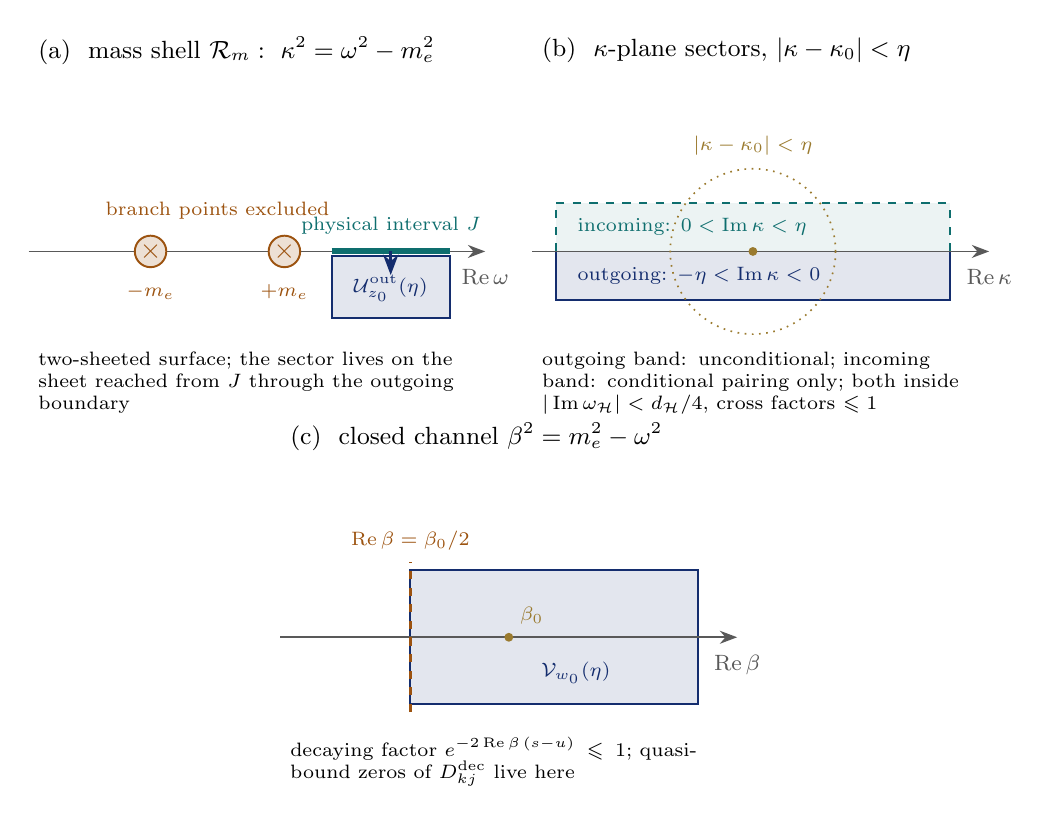
\begin{tikzpicture}[x=1cm,y=1cm]

% ============ panel (a): energy plane of the mass shell R_m ================
\begin{scope}[shift={(0,0)}]
  \node[lab, anchor=west] at (-0.4,2.55) {(a)\ \ mass shell $\mathcal R_m:\ \kappa^2=\omega^2-m_e^2$};
  \draw[axis] (-0.4,0) -- (5.4,0) node[slab, anchor=north, yshift=-1mm] {$\operatorname{Re}\omega$};
  % threshold branch points, excluded disks
  \foreach \x/\l in {1.15/{-m_e}, 2.85/{+m_e}}{
    \draw[warm, fill=warm!18, line width=0.7pt] (\x,0) circle (0.20);
    \node[warm] at (\x,0) {$\times$};
    \node[tlab, warm, anchor=north] at (\x,-0.30) {$\l$};}
  \node[tlab, warm, anchor=south] at (2.0,0.28) {branch points excluded};
  % physical interval J and the outgoing sector below it
  \draw[chI, line width=2.2pt] (3.45,0) -- (4.95,0);
  \node[tlab, chI, anchor=south] at (4.2,0.10) {physical interval $J$};
  \fill[chH!12] (3.45,-0.06) rectangle (4.95,-0.85);
  \draw[chH, line width=0.7pt] (3.45,-0.06) rectangle (4.95,-0.85);
  \node[tlab, chH] at (4.2,-0.47) {$\mathcal U^{\rm out}_{z_0}(\eta)$};
  \draw[outarr, chH] (4.2,0.0) -- (4.2,-0.30);
  \node[tlab, anchor=north west, text width=5.6cm] at (-0.4,-1.15)
    {two-sheeted surface; the sector lives on the sheet reached from $J$
     through the outgoing boundary};
\end{scope}

% ============ panel (b): kappa-plane one-sided sectors ======================
\begin{scope}[shift={(6.4,0)}]
  \node[lab, anchor=west] at (-0.4,2.55) {(b)\ \ $\kappa$-plane sectors, $|\kappa-\kappa_0|<\eta$};
  % bands
  \fill[chH!12] (-0.1,-0.62) rectangle (4.9,0);
  \draw[chH, line width=0.7pt] (-0.1,-0.62) rectangle (4.9,0);
  \fill[chI!8] (-0.1,0) rectangle (4.9,0.62);
  \draw[chI, line width=0.7pt, dashed] (-0.1,0.62) -- (4.9,0.62)
    (-0.1,0) -- (-0.1,0.62) (4.9,0) -- (4.9,0.62);
  \draw[axis] (-0.4,0) -- (5.4,0) node[slab, anchor=north, yshift=-1mm] {$\operatorname{Re}\kappa$};
  \fill[acc] (2.4,0) circle (1.6pt);
  \node[tlab, acc, anchor=south] at (2.4,1.10) {$|\kappa-\kappa_0|<\eta$};
  \draw[acc, dotted, line width=0.6pt] (2.4,0) circle (1.05);
  \node[tlab, chH, anchor=west] at (0.05,-0.31)
    {outgoing: $-\eta<\operatorname{Im}\kappa<0$};
  \node[tlab, chI, anchor=west] at (0.05,0.31)
    {incoming: $0<\operatorname{Im}\kappa<\eta$};
  \node[tlab, anchor=north west, text width=5.6cm] at (-0.4,-1.15)
    {outgoing band: unconditional; incoming band: conditional pairing only;
     both inside $|\operatorname{Im}\omega_{\mathcal H}|<d_{\mathcal H}/4$,
     cross factors $\leqslant1$};
\end{scope}

% ============ panel (c): closed-channel beta half-plane =====================
\begin{scope}[shift={(3.2,-4.9)}]
  \node[lab, anchor=west] at (-0.4,2.55) {(c)\ \ closed channel $\beta^2=m_e^2-\omega^2$};
  \fill[chH!12] (1.25,-0.85) rectangle (4.9,0.85);
  \draw[chH, line width=0.7pt] (1.25,-0.85) rectangle (4.9,0.85);
  \draw[axis] (-0.4,0) -- (5.4,0) node[slab, anchor=north, yshift=-1mm] {$\operatorname{Re}\beta$};
  \draw[warm, line width=0.8pt, dashed] (1.25,-0.95) -- (1.25,0.95);
  \node[tlab, warm, anchor=south] at (1.25,0.98) {$\operatorname{Re}\beta=\beta_0/2$};
  \fill[acc] (2.5,0) circle (1.6pt);
  \node[tlab, acc, anchor=south west] at (2.52,0.04) {$\beta_0$};
  \node[tlab, chH] at (3.35,-0.45) {$\mathcal V_{w_0}(\eta)$};
  \node[tlab, anchor=north west, text width=5.6cm] at (-0.4,-1.15)
    {decaying factor $e^{-2\operatorname{Re}\beta\,(s-u)}\leqslant1$;
     quasi-bound zeros of $D^{\rm dec}_{kj}$ live here};
\end{scope}

\end{tikzpicture}
\end{document}
